\documentclass[18pt,oneside,a4paper, titlepage]{article}

\usepackage[hidelinks]{hyperref}
\usepackage[pdftex]{graphicx}
\usepackage{adjustbox}

\begin{document}
\begin{figure}[t]
	\centering
	
\includegraphics[scale=0.35]{logo-polimi.png}
\end{figure}
\title{\textbf{myTaxiService}\\\textbf{I}ntegration \textbf{T}est \textbf{P}lan \textbf{D}ocument\\ A.Y. 2015/2016\\
	Politecnico di Milano \\ Version 1.0}	
\author{Cattaneo Michela Gaia, matr. 791685\\Barlocco Mattia, matr. 792735 }
\date{January 22, 2016}
\maketitle

\newpage
	\tableofcontents

\newpage
\section{Introduction}
	\subsection{Revision History}
		% Record all revisions to the document.
	\subsection{Purpose	and	Scope}
		% State	the	purpose	and	scope of the document.
		\subsubsection{Purpose}
		This document represents the Integration Test Plan Document. It aims at specifying the plan for the integration testing of myTaxiService application, ensuring that all its modules interacts properly. There are also specifications about the integration strategy and the sequence of the integration of the components of the system already defined, along with an justification of the tools that are needed for the testing.\\
		This document is intended for the development team, that needs to know what it is needed to test, in which sequence it should occur and with which tools.
		\subsubsection{Scope}
		myTaxiService is an application that simplifies the access of the customers to the taxi service, managing also the taxi driver's distribution over the city and the queues of the areas. The customer can use the mobile application or the web app to request or reserve a taxi and a notification is forwarded to the designated taxi driver, who is going to answer.\\ This system should always be responsive and reliable, in order to keep up with all the requests of the passenger and the notifications forwarding.\\ This is the reason why the components that comprise the myTaxiService system are meant to be well integrated and tested.
	\subsection{List of	Definitions	and	Abbreviations}
		\begin{itemize}
			\item \textbf{Definitions}
			\item[-] \textbf{Passenger}: a person who is registered in the application.
			\item[-] \textbf{Taxi driver}: a taxi driver who access the application with a specific ID.
			\item[-] \textbf{Request}: the request of a taxi in a certain area and position in the city made by a user.
			\item[-] \textbf{Reservation}: the reservation of a taxi in a certain area, place and time that can be made only by passengers.
			\item[-] \textbf{Component}: a modular part of a system with encapsulated content and whose manifestation is replaceable within its environment.
			\item[-] \textbf{Subsystem}: a behavioral unit in the physical system, and hence in the model.
		\newpage	
			\item \textbf{Acronyms and abbreviations}
			\item[-] \textbf{RASD}: Requirement Analysis and Specification Document
			\item[-] \textbf{DD}: Design Document
			\item[-] \textbf{JEE}: Java Enterprise Edition
			\item[-] \textbf{JVM}: Java Virtual Machine
			
		\end{itemize}
	\subsection{List of	Reference Documents}
		%	List	all	reference	documents,	for	instance:
		%• The	project	description
		%• The	RASD
		%• The	Design	document
		%• The	documentation	of	any	tool	you	plan	to	use	for	testing
		\begin{itemize}
			\item Project Description and Rules (\url{https://github.com/MichelaCattaneo/myTaxiService/blob/master/Project\%20Description\%20And\%20Rules.pdf})
			\item Requirements Analysis and Specification Document (\url{https://github.com/MichelaCattaneo/myTaxiService/blob/master/Deliveries/RASD_1.1.pdf})
			\item Design Document (\url{https://github.com/MichelaCattaneo/myTaxiService/blob/master/Deliveries/DD.pdf})
			\item Integration Test Plan Example (\url{https://beep.metid.polimi.it/documents/3343933/5b3768d0-­‐‑d949-­‐‑4369-­‐‑87e1-­‐‑7a31b6943726})
		\end{itemize}

\newpage
\section{Integration Strategy}
	\subsection{Entry Criteria}	
		These are the criteria that must be respected before the integration testing phase may begin:
		\begin{itemize}
			\item Requirement Analysis and Specification Document is complete and revised
			\item Design Document is complete and revised
			\item Code Inspection Document is complete and revised
			\item The code is complete and high prioritized bugs fixed
			\item The product satisfies the requirements and the assumptions specified in the RASD
			\item The product satisfies the architecture and the design specified in the DD
			\item Test environment, test cases and test data are ready
		\end{itemize}	
		% Specify	the	criteria	that	must	be	met	before	integration testing of specific	elements	may	begin	(e.g.,	functions	must	have	been	unit tested).
	\newpage
	\subsection{Elements to	be Integrated}
		%Identify	the	components	to	be	integrated,	refer	to	your design	document	to	identify	such	components	in	a	way	that	is	consistent with	your	design.
		These components refer to the ones specified in the Component View in chapter 2.3 of the DD. This diagram shows how these components have to be integrated and the order of integration, according to the strategy adopted.
		
		\vspace{0.5cm}
		
		\begin{figure}[h]
			\centering
			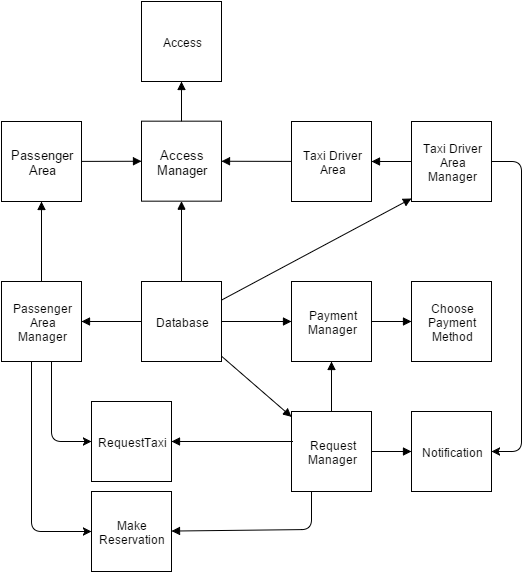
\includegraphics[scale=0.6]{ElementsToBeIntegrated.png}
		\end{figure}
		
		\vspace{0.5cm}
	\subsection{Integration Testing Strategy}
		% Describe	the	integration testing approach (top-down,	bottom-up,functional	groupings,	etc.)	and	the	rationale for	the	choosing that approach.
		The integration testing strategy that has been chosen exploits the bottom-up approach. This strategy is the most suitable for the myTaxiService system, in fact it makes it easier to find bugs, starting from the most critical components. The bottom-up approach starts from the lowest layers of the system, testing the basic functionalities at the beginning, then moving forward the most abstract layers, such as the client interfaces modules.\\ In this case, it is only necessary to use drivers, in order to simulate the top layers during the testing, which are a lot easier to produce with respect to the stubs used in the top-down approach.
	\newpage
	\subsection{Sequence of	Component/Function Integration}
		% NOTE:	 The structure	of	this	section	may	vary	depending	on	the	integration	strategy	you	select	in	Section	2.3. Use the structure proposed	below	as	a	non	mandatory	guide.	
		\subsubsection{Software	Integration	Sequence}
		% For	each	subsystem: Identify	the	sequence	in	which	the	software	components will	be	integrated within	the	subsystem.	Relate	this	sequence	to	any	product	features/functions	that	are	being	built	up.	
			In this section the system is presented already divided in the main three subsystems: Manager, Taxi Driver Client and Passenger Client.
			\begin{itemize}
				
				
				\item \textbf{Integration Test of the "Manager" subsystem }
					\vspace{0.5cm}
					\begin{center}
						\centering
						\begin{tabular}{c c c}
							\hline \textbf{ID} & \textbf{Integration Test} & \textbf{Paragraph} \\
							\hline		I1 &  Database $\rightarrow$ AccessManager & \hyperlink{chapter 3.1}{3.1}\\
							\hline		I2 & Database $\rightarrow$ TaxiDriverAreaManager & \hyperlink{chapter 3.2}{3.2} \\
							\hline		I3 & Database $\rightarrow$ PassengerAreaManager & \hyperlink{chapter 3.3}{3.3}\\
							\hline		I4 & Database $\rightarrow$ RequestManager & \hyperlink{chapter 3.4}{3.4} \\
							\hline		I5 & Database $\rightarrow$ PaymentManager & \hyperlink{chapter 3.5}{3.5} \\
							\hline
						\end{tabular}
					\end{center}
					
					
					\begin{figure}[h]
						\centering
						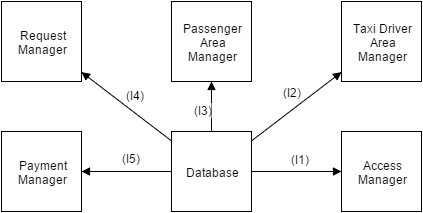
\includegraphics[scale=0.5]{ManagerSubsystem.png}
					\end{figure}
					
					\vspace{1cm}
					
				\item \textbf{Integration Test of the "Taxi Driver Client" subsystem }
					
					\vspace{0.5cm}
					\begin{center}
						\centering
						\begin{tabular}{c c c}
							\hline \textbf{ID} & \textbf{Integration Test} & \textbf{Paragraph} \\
							\hline		I6T1 & RequestManager $\rightarrow$ Notification & \hyperlink{chapter 3.6}{3.6}\\
							\hline		I6T2 & TaxiDriverAreaManager $\rightarrow$ Notification & \hyperlink{chapter 3.6}{3.6} \\
							\hline		I7T1 & TaxiDriverAreaManager $\rightarrow$ TaxiDriverArea & \hyperlink{chapter 3.7}{3.7}\\
							\hline		I7T2 & AccessManager $\rightarrow$ TaxiDriverArea & \hyperlink{chapter 3.7}{3.7} \\
							\hline		I8 & AccessManager $\rightarrow$ Access (Taxi Driver) & \hyperlink{chapter 3.8}{3.8} \\
							\hline
						\end{tabular}
					\end{center}
					
					\begin{figure}[h]
						\centering
						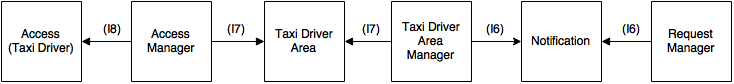
\includegraphics[scale=0.49]{TaxiDriverSubsystem.png}
					\end{figure}
				\newpage
				\item \textbf{Integration Test of the "Passenger Client" subsystem}
				
					\vspace{0.5cm}
					\begin{center}
						\centering
						\begin{tabular}{c c c}
							\hline \textbf{ID} & \textbf{Integration Test} & \textbf{Paragraph} \\
							\hline		I9 & RequestManager $\rightarrow$ PaymentManager & \hyperlink{chapter 3.9}{3.9}\\
							\hline		I10T1 & RequestManager $\rightarrow$ MakeReservation & \hyperlink{chapter 3.10}{3.10} \\
							\hline		I10T2 & PassengerAreaManager $\rightarrow$ MakeReservation & \hyperlink{chapter 3.10}{3.10}\\
							\hline		I11T1 & RequestManager $\rightarrow$ RequestTaxi & \hyperlink{chapter 3.11}{3.11}\\
							\hline		I11T2 & PassengerAreaManager $\rightarrow$ RequestTaxi & \hyperlink{chapter 3.11}{3.11} \\
							\hline		I12T1 & PassengerAreaManager $\rightarrow$ PassengerArea & \hyperlink{chapter 3.12}{3.12} \\
							\hline		I12T2 & AccessManager $\rightarrow$ PassengerArea & \hyperlink{chapter 3.12}{3.12}\\
							\hline		I13 & AccessManager $\rightarrow$ Access (Passenger) & \hyperlink{chapter 3.13}{3.13} \\
							\hline		I14 & PaymentManager $\rightarrow$ ChoosePaymentMethod & \hyperlink{chapter 3.14}{3.14} \\
							\hline
						\end{tabular}
					\end{center}
					
					
					\begin{figure}[h]
						\centering
						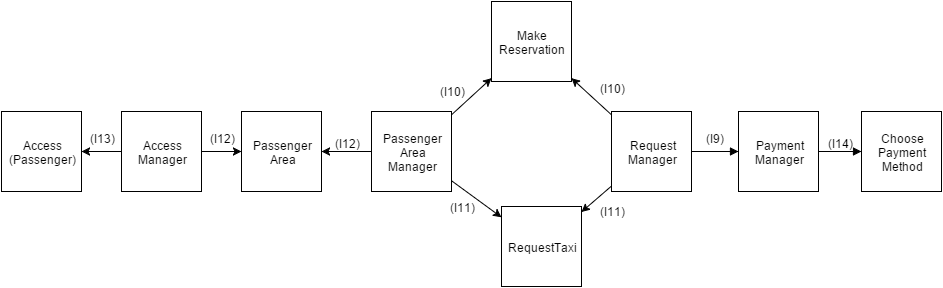
\includegraphics[scale=0.4]{PassengerSubsystem.png}
					\end{figure}
			\end{itemize}
			\vspace{1cm}
			
		\subsubsection{Subsystem Integration Sequence}
			% Identify	the	order	in which	subsystems	will	be	integrated. If	you	have	a	single	subsystem,	2.4.1	and	2.4.2	are	to	be	merged	in a	single	section.	You	can	refer	to	Section	2.2	of	the	test	plan example [1] as	an	example	of	what	we	expect.
			
			The subsystems will be integrated in this order:
			\begin{enumerate}
				\item \textbf{Manager}: According to the strategy adopted, this is the first subsystem that is going to be integrated, as it is the lowest level of the myTaxiService system. It is necessary to test this part first, as long as this part manages the other components and it is crucial that this part does integrates perfectly with the others.
				\item \textbf{Taxi Driver Client}: This is the second subsystem that will be integrated.
				\item \textbf{Passenger Client}: This is the last subsystem that will be integrated.
			\end{enumerate}
			There is no real need to test the taxi driver client before or after the passenger client, as they are both top level modules that have to be integrated in the last steps. 
		

\newpage

\documentclass[18pt,oneside,a4paper, titlepage]{article}

\usepackage[hidelinks]{hyperref}
\usepackage[pdftex]{graphicx}

\begin{document}
\section{Individual	Steps	and	Test	Description}
	\subsection{Integration Test case I1}
		\begin{tabular}{ l l}
			\hline 		\textbf{Test case identifier} & I1 \\
			\hline		\textbf{Test item(s)}  & Database $\rightarrow$ AccessManager \\
			\hline		\textbf{Input specification} & The database sends to the AccessManager the data \\ & that it has requested by a query or by an INSERT \\ & or by an UPDATE. \\
			\hline		\textbf{Output specification} & Check if the INSERT and UPDATE have been done\\ & correctly, check if the result of the query is what\\ &  we expect and check if the result is computed correctly\\ & by the AccessManager.\\
			\hline		\textbf{Environmental needs} & Database data available.\\
			\hline
		\end{tabular}
	\subsection{Integration Test case I2}
		\begin{tabular}{ l l}
			\hline 		\textbf{Test case identifier} & I2 \\
			\hline		\textbf{Test item(s)}  & Database $\rightarrow$ TaxiDriverAreaManager \\
			\hline		\textbf{Input specification} & The database sends to the TaxiDriverAreaManager the\\ & data that it has requested by a query or by an INSERT \\ & or by an UPDATE.\\
			\hline		\textbf{Output specification} &  Check if the INSERT and UPDATE have been done\\ & correctly, check if the result of the query is what\\ &  we expect and check if the result is computed correctly\\ & by the TaxiDriverAreaManager.\\
			\hline		\textbf{Environmental needs} & Database data available.\\
			\hline
		\end{tabular}
	\subsection{Integration Test case I3}
		\begin{tabular}{ l l}
			\hline 		\textbf{Test case identifier} & I3 \\
			\hline		\textbf{Test item(s)}  & Database $\rightarrow$ PassengerAreaManager \\
			\hline		\textbf{Input specification} & The database sends to the PassengerAreaManager the\\ & data that it has requested by a query or by an INSERT \\ & or by an UPDATE.\\
			\hline		\textbf{Output specification} & Check if the INSERT and UPDATE have been done\\ & correctly, check if the result of the query is what\\ &  we expect and check if the result is computed correctly\\ & by the PassengerAreaManager.\\
			\hline		\textbf{Environmental needs} &  Database data available.\\
			\hline
		\end{tabular}
	\subsection{Integration Test case I4}
		\begin{tabular}{ l l}
			\hline 		\textbf{Test case identifier} & I4 \\
			\hline		\textbf{Test item(s)}  & Database $\rightarrow$ RequestManager \\
			\hline		\textbf{Input specification} & The database sends to the RequestManager the data\\ & that it has requested by a query or by an INSERT \\ & or by an UPDATE.\\
			\hline		\textbf{Output specification} &  Check if the INSERT and UPDATE have been done\\ & correctly, check if the result of the query is what\\ &  we expect and check if the result is computed correctly\\ & by the RequestManager.\\
			\hline		\textbf{Environmental needs} & Database data available.\\
			\hline
		\end{tabular}
	\subsection{Integration Test case I5}
		\begin{tabular}{ l l}
			\hline 		\textbf{Test case identifier} & I5 \\
			\hline		\textbf{Test item(s)}  & Database $\rightarrow$ PaymentManager \\
			\hline		\textbf{Input specification} & The database sends to the PaymentManager the data\\ & that it has requested by a query or by an INSERT \\ & or by an UPDATE.\\
			\hline		\textbf{Output specification} &  Check if the INSERT and UPDATE have been done\\ & correctly, check if the result of the query is what\\ &  we expect and check if the result is computed correctly\\ & by the PaymentManager.\\
			\hline		\textbf{Environmental needs} & Database data available.\\
			\hline
		\end{tabular}
	\subsection{Integration Test case I6}
		\begin{tabular}{ l l}
			\hline 		\textbf{Test case identifier} & I6 \\
			\hline		\textbf{Test item(s)}  & PaymentManager $\rightarrow$ RequestManager \\
			\hline		\textbf{Input specification} & The PaymentManager sends to the RequestManager the \\ & data about how the Passenger wants to pay the ride.\\
			\hline		\textbf{Output specification} & Check if the Payment method is managed correctly.\\
			\hline		\textbf{Environmental needs} & I5 succeeded\\
			\hline
		\end{tabular}
	\subsection{Integration Test case I7}
		\begin{tabular}{ l l}
			\hline 		\textbf{Test case identifier} & I7 \\
			\hline		\textbf{Test item(s)}  & RequestManager $\rightarrow$ Notification \\
			\hline		\textbf{Input specification} & The RequestManager sends to the Notification all \\ & the notifies of a specific Taxi driver.\\
			\hline		\textbf{Output specification} & Check if the notifies are of the correct Taxi driver.\\
			\hline		\textbf{Environmental needs} & I4 succeeded\\
			\hline
		\end{tabular}
	\subsection{Integration Test case I8}
		\begin{tabular}{ l l}
			\hline 		\textbf{Test case identifier} & I8 \\
			\hline		\textbf{Test item(s)}  & Notification $\rightarrow$ TaxiDriverArea \\
			\hline		\textbf{Input specification} & The Notification sends an alert message to the \\ & TaxiDriverArea if a notify is detected.\\
			\hline		\textbf{Output specification} & Check if the message is computed correctly by the\\ & TaxiDriverArea.\\
			\hline		\textbf{Environmental needs} & I7 succeeded\\
			\hline
		\end{tabular}
	\subsection{Integration Test case I9}
		\begin{tabular}{ l l}
			\hline 		\textbf{Test case identifier} & I9 \\
			\hline		\textbf{Test item(s)}  & TaxiDriverAreaManager $\rightarrow$ TaxiDriverArea \\
			\hline		\textbf{Input specification} & The TaxiDriverAreaManager sends to the TaxiDriverArea\\ & the profile information of the Taxi driver requested.\\
			\hline		\textbf{Output specification} & Check if the correct information have been sent.\\
			\hline		\textbf{Environmental needs} & I2 succeeded\\
			\hline
		\end{tabular}
	\subsection{Integration Test case I10}
		\begin{tabular}{ l l}
			\hline 		\textbf{Test case identifier} & I10 \\
			\hline		\textbf{Test item(s)}  & AccessManager $\rightarrow$ TaxiDriverArea \\
			\hline		\textbf{Input specification} & The AccessManager sends to the TaxiDriverArea the\\ & identification data of the Taxi driver logged in.\\
			\hline		\textbf{Output specification} & Check if the TaxiDriverArea has built the profile\\ & page of the correct Taxi driver logged in.\\
			\hline		\textbf{Environmental needs} & I9 succeeded\\
			\hline
		\end{tabular}
	\subsection{Integration Test case I11}
		\begin{tabular}{ l l}
			\hline 		\textbf{Test case identifier} & I11 \\
			\hline		\textbf{Test item(s)}  & Access $\rightarrow$ AccessManager \\
			\hline		\textbf{Input specification} & The Access sends to the AccessManager the data\\ & that the client has inserted in the input form of \\ & the registration or the log in.\\
			\hline		\textbf{Output specification} & Check if the AccessManager computes the inputs\\ & correctly.\\
			\hline		\textbf{Environmental needs} & I1 succeeded\\
			\hline
		\end{tabular}
	\subsection{Integration Test case I12}
		\begin{tabular}{ l l}
			\hline 		\textbf{Test case identifier} & I12 \\
			\hline		\textbf{Test item(s)}  & PaymentManager $\rightarrow$ ChoosePaymentMethod \\
			\hline		\textbf{Input specification} & The PaymentManager sends to the ChoosePaymentMethod \\ & the data of the Passenger's credit card.\\
			\hline		\textbf{Output specification} & Check if the ChoosePaymentMethod computes the inputs \\ & correctly.\\
			\hline		\textbf{Environmental needs} & I5 succeeded\\
			\hline
		\end{tabular}
	\subsection{Integration Test case I13}
		\begin{tabular}{ l l}
			\hline 		\textbf{Test case identifier} & I13 \\
			\hline		\textbf{Test item(s)}  & ChoosePaymentMethod $\rightarrow$ RequestManager \\
			\hline		\textbf{Input specification} & The ChoosePaymentMethod sends to the \\ & RequestManager the choice of the Passenger.\\
			\hline		\textbf{Output specification} & Check if the RequestManager computes the\\ & input correctly.\\
			\hline		\textbf{Environmental needs} & I12 succeeded\\
			\hline
		\end{tabular}
	\subsection{Integration Test case I14}
		\begin{tabular}{ l l}
			\hline 		\textbf{Test case identifier} & I14 \\
			\hline		\textbf{Test item(s)}  & RequestManager $\rightarrow$ MakeReservation \\
			\hline		\textbf{Input specification} & The RequestManager searches a taxi for a reservation\\ & and it sends to the MakeReservation the results.\\
			\hline		\textbf{Output specification} & Check if the MakeReservation computes the inputs\\ & correctly.\\
			\hline		\textbf{Environmental needs} & I4 succeeded\\
			\hline
		\end{tabular}
	\subsection{Integration Test case I15}
		\begin{tabular}{ l l}
			\hline 		\textbf{Test case identifier} & I15 \\
			\hline		\textbf{Test item(s)}  & RequestManager $\rightarrow$ RequestTaxi \\
			\hline		\textbf{Input specification} & The RequestManager searches a taxi for a reservation\\ & and it sends to the RequestTaxi the results.\\
			\hline		\textbf{Output specification} & Check if the RequestTaxi computes the inputs\\ & correctly.\\
			\hline		\textbf{Environmental needs} & I4 succeeded\\
			\hline
		\end{tabular}
	\subsection{Integration Test case I16}
		\begin{tabular}{ l l}
			\hline 		\textbf{Test case identifier} & I16 \\
			\hline		\textbf{Test item(s)}  & RequestTaxi $\rightarrow$ PassengerArea \\
			\hline		\textbf{Input specification} & The RequestTaxi sends an alert message to the\\ & PassengerArea when a taxi is found.\\
			\hline		\textbf{Output specification} & Check if the PassengerArea computes the message\\ & correctly.\\
			\hline		\textbf{Environmental needs} & I15 succeeded\\
			\hline
		\end{tabular}
	\subsection{Integration Test case I17}
		\begin{tabular}{ l l}
			\hline 		\textbf{Test case identifier} & I17 \\
			\hline		\textbf{Test item(s)}  & MakeReservation $\rightarrow$ PassengerArea \\
			\hline		\textbf{Input specification} & The MakeReservation sends an alert message to the\\ & PassengerArea when a taxi is found.\\
			\hline		\textbf{Output specification} &  Check if the PassengerArea computes the message\\ & correctly.\\
			\hline		\textbf{Environmental needs} & I14 succeeded\\
			\hline
		\end{tabular}
	\subsection{Integration Test case I18}
		\begin{tabular}{ l l}
			\hline 		\textbf{Test case identifier} & I18 \\
			\hline		\textbf{Test item(s)}  & PassengerAreaManager $\rightarrow$ PassengerArea \\
			\hline		\textbf{Input specification} & The PassengerAreaManager sends to the PassengerArea\\ & the profile information of the Passenger requested.\\
			\hline		\textbf{Output specification} & Check if the correct information have been sent.\\
			\hline		\textbf{Environmental needs} & I3 succeeded\\
			\hline
		\end{tabular}
	\subsection{Integration Test case I19}
		\begin{tabular}{ l l}
			\hline 		\textbf{Test case identifier} & I19 \\
			\hline		\textbf{Test item(s)}  & AccessManager $\rightarrow$ PassengerArea \\
			\hline		\textbf{Input specification} &  The AccessManager sends to the PassengerArea the\\ & identification data of the Passenger logged in.\\
			\hline		\textbf{Output specification} & Check if the PassengerArea has built the profile\\ & page of the correct Passenger logged in.\\
			\hline		\textbf{Environmental needs} & I1 succeeded\\
			\hline
		\end{tabular}
	\subsection{Integration Test case I20}
		\begin{tabular}{ l l}
			\hline 		\textbf{Test case identifier} & I20 \\
			\hline		\textbf{Test item(s)}  & Access $\rightarrow$ AccessManager \\
			\hline		\textbf{Input specification} & The Access sends to the AccessManager the data\\ & that the client has inserted in the input form of \\ & the registration or the log in.\\
			\hline		\textbf{Output specification} & Check if the AccessManager computes the inputs\\ & correctly.\\
			\hline		\textbf{Environmental needs} & I19 succeeded\\
			\hline
		\end{tabular}
\end{document}
	% For	each	step	of	the	integration	process	identified	above,	describe	the	 type	of	tests	that	will	be	used	to	verify	that	the	elements	integrated	in	this step	perform	as	expected.	Describe	in general	the	expected	results	of	the	 test	set.	You	may	refer	to	Chapter	3	and	Chapter	4	of	the	test	plan example	[1]	as	an	example	of	what	we	expect. (NOTE:	This	is	not	a	detailed	description	of	test	protocols.	Think	of	this	as the	test	design	phase.	Specific	protocols	will	be	written	to	fulfill	the	goals of	the	tests	identified	in	this	section.)

\newpage
\section{Tools	and	Test	Equipment	Required}
	% Identify	all	tools	and	test	equipment	needed	to	accomplish	the	 integration.	Refer	to	the	tools	presented	during	the	lectures.	Explain	why	 and	how	you	are	going	to	use	them.	Note	that	you	may	also	use	manual	testing	for	some	part.	Consider manual	testing	as	one	of	the	possible	tools	you	have	available.
	\subsection{Unit Testing and JUnit}
		Integration testing is usually performed after unit testing has been finished. Unit testing is usually done in the first part of the development and, once all the individual units are created and tested, it is necessary to start combining these modules one by one and test their behavior as a combined unit.\\
		Therefore, unit testing is done in order to already have a visual feedback and all the possible problems sorted out, but all the classes are tested separately, so it will be necessary to check if they integrate properly with an integration testing afterwards.\\
		In fact, in this phase all the classes are tested with each test case independent from the others, allowing to find both bugs in the programmer's implementation and flaws or missing parts of the specification. \\
		JUnit is a unit testing framework for the Java programming language and is the tool usually used for performing unit testing. It will be employed to write and run repeatable tests on the classes and methods of the myTaxiService application.
		
	\subsection{Mockito}
		In unit testing, mock objects can simulate the behavior of complex, real objects, so they are useful when a real object is impractical or impossible to incorporate into a unit test.\\ They are also useful, as they allow developers to focus their tests on the behavior of the system without worrying about its dependencies and having a predictable results.\\
		A tool that can be exploited is Mockito, a simple mocking framework widely used for Java, to create unit testing mockups. \\
		It will be used for producing mock objects out of the Database component, or out of objects that supplies non-deterministic results or whose states are difficult to reproduce.
	
	\subsection{Arquillian and ShrinkWrap.}
		Arquillian is an innovative, highly extensible and flexible testing platform for the JVM.\\ It enables developers to easily create automated integration, functional and acceptance tests for Java middlewares. \\In fact it combines a unit testing framework (JUnit or TestNG), ShrinkWrap, and one or more supported target containers (Java EE container, servlet container, etc) to provide a simple, flexible and pluggable integration testing environment, with no need of any special configuration.
	\newpage
	\noindent
		Its extensibility can be found in the different modules and extension it offers, that provide very useful functionalities for every aspect of the software system.
		\vspace{0.5cm}
		\begin{figure}[h]
			\centering
			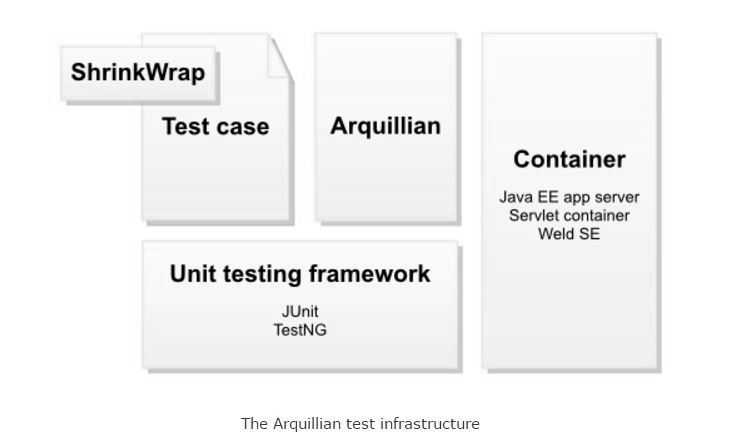
\includegraphics[scale=0.45]{Arquillian.jpg}
		\end{figure}
			
		\vspace{0.5cm}
	
		Arquillian will be mainly used for:
		\begin{itemize}
			\item Managing the lifecycle of one or more containers
			\item Bundling the test case, dependent classes and resources into a ShrinkWrap archive
			\item Deploying the archive to the container
			\item Enriching the test case by providing dependency injection and other declarative services
			\item Executing the tests inside (or against) the container
			\item Capturing the results and returning them to the test runner for reporting
		\end{itemize}
		
			
		\vspace{0.5cm}
			
		ShrinkWrap is the simplest way to create and define custom archives in Java, that encapsulate the test class and its dependent resources, powering the Arquillian deployment mechanism. In fact, the test case is dispatched to the container's environment through coordination with ShrinkWrap: Arquillian packages the ShrinkWrap-defined archive at runtime and deploys it to the target container.
		
	\subsection{Manual testing.}
		Manual testing can be considered a valid solution, depending on the application to be tested.\\ In this case a tester ensures the correct behaviors of the components, by following a test plan that allows him to find the most important use cases, without any support from tools or scripts.\\ This is used in alternative of the automated tests, which is more quickly, less expensive and more accurate, because in some particular scenarios it is necessary to exploit human observation, logic and experience.

\newpage
\section{Program	Stubs	and	Test	Data	Required}
	% Based	on	the	testing	strategy	and	test	design,	identify	any	program	stubs or	special	test	data	required	for	each	integration	step.
	Here is presented the drivers used for the simulation of the interfaces, essentials for testing the integration between them and the other components.
	\subsection{Notification driver}
		This driver simulates the behaviour of the Notification component.\\ Its duty is to receive the notifications of the taxi driver that wants to see this panel in his taxi driver area. Moreover, it receives and displays the notifications managed by the TaxiDriverAreaManager, when he is selected for a taxi request by a passenger.
	\subsection{TaxiDriverArea driver}
		This driver simulates the behaviour of the TaxiDriverArea component.\\ Once the taxi driver requests it, the TaxiDriverArea receives the profile information sent from the TaxiDriverAreaManager and the identification data sent from the AccessManager when he logs in.
	\subsection{Access driver}
		This driver simulates the behaviour of the Access component.\\ This driver simulates the registration or log in of a passenger or of a taxi driver, sending the data of the input form to the AccessManager, in order to see if it can compute them properly.
	\subsection{PassengerArea driver}
		This driver simulates the behaviour of the PassengerArea component.\\ When the passenger wants to see or edit his profile, the PassengerAreaManager sends the profile information to the PassengerArea, so that it can display it. Additionally, it receives from the AccessManager the identification data of a user that has just logged in, so that it can display his personal area.
	\subsection{MakeReservation driver}
		This driver simulates the behaviour of the MakeReservation component.\\ The RequestManager expects from this component the data of the input form of the reservation, checking if the information inserted is correct. It also displays the reservation data in the passenger area, sending them to the PassengerAreaMananger right after the reservation has been done.
	\subsection{RequestTaxi driver}
		This driver simulates the behaviour of the RequestTaxi component.\\ It receives the result of the search of a taxi made from the RequestManager and the previous requests are displayed in the passenger personal area, once they are sent to the PassengerAreaManager.
	\subsection{ChoosePaymentMethod driver}
		This driver simulates the behaviour of the ChoosePaymentMethod component.\\ The passenger chooses the payment method he prefers and the answer is sent to the PaymentManager.
	\newpage
	\section{Appendix}
	\subsection{Software and tool used}
		\begin{itemize}
			\item TeXstudio (\url{http://www.texstudio.org/}): to redact and to format this document.
			\item draw.io (\url{https://www.draw.io/}):to create diagrams of the components to be integrated.
		\end{itemize}
	
	\subsection{Hours of work}
		Time spent redacting this document:
		\begin{itemize}
			\item Cattaneo Michela Gaia: {\raise.17ex\hbox{$\scriptstyle\sim$}}10 hours of work.
			\item Barlocco Mattia: {\raise.17ex\hbox{$\scriptstyle\sim$}}10 hours of work.
		\end{itemize}

\end{document}